% Source: AESP_466_ClassWork/Supplements/Companion/Euler_Sequences_Quaternions/Euler_Sequences_Quaternions.tex

\documentclass[border=4pt]{standalone}
\usepackage{amsmath}
\usepackage{amssymb}
\usepackage{graphicx}
\usepackage{tikz}
\usepackage{xcolor}
\usetikzlibrary{shapes.geometric, arrows.meta, positioning, decorations.pathmorphing, decorations.pathreplacing, patterns, calc, 3d}

\definecolor{Garnet}{HTML}{73000A}
\definecolor{USC_Rose}{HTML}{CC2E40}
\definecolor{USC_Blue}{HTML}{466A9F}
\definecolor{USC_Slate}{HTML}{1F414D}
\definecolor{USC_Olive}{HTML}{65780B}
\definecolor{USC_Lime}{HTML}{CED318}
\definecolor{USC_Gold}{HTML}{A49137}
\definecolor{USC_Black90}{HTML}{565656}
\definecolor{USC_Black10}{HTML}{ECECEC}

\newcommand{\sectionheader}[1]{%
  \vspace{0.5cm}
  {\noindent\Large \textbf{#1}}
  \vspace{0.2cm}
  \hrule
  \vspace{0.1cm}
  \hrule
  \vspace{0.3cm}
}

\begin{document}
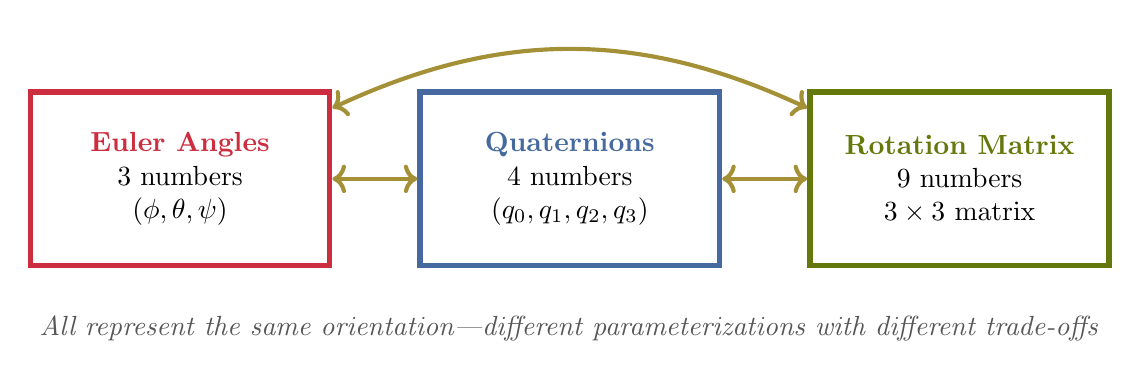
\begin{tikzpicture}[scale=0.9]
    % Three boxes showing representations - using solid borders with white fill
    \node[draw=USC_Rose, line width=2pt, fill=white, minimum width=3.8cm, minimum height=2.2cm, sharp corners, align=center] (euler) at (0,0) {\textbf{\textcolor{USC_Rose}{Euler Angles}}\\3 numbers\\$(\phi, \theta, \psi)$};
    \node[draw=USC_Blue, line width=2pt, fill=white, minimum width=3.8cm, minimum height=2.2cm, sharp corners, align=center] (quat) at (5.5,0) {\textbf{\textcolor{USC_Blue}{Quaternions}}\\4 numbers\\$(q_0, q_1, q_2, q_3)$};
    \node[draw=USC_Olive, line width=2pt, fill=white, minimum width=3.8cm, minimum height=2.2cm, sharp corners, align=center] (dcm) at (11,0) {\textbf{\textcolor{USC_Olive}{Rotation Matrix}}\\9 numbers\\$3 \times 3$ matrix};

    % Arrows with USC colors
    \draw[<->, line width=1.5pt, USC_Gold] (euler) -- (quat);
    \draw[<->, line width=1.5pt, USC_Gold] (quat) -- (dcm);
    \draw[<->, line width=1.5pt, USC_Gold, bend left=25] (euler) to (dcm);

    \node[below, USC_Black90] at (5.5,-1.8) {\textit{All represent the same orientation---different parameterizations with different trade-offs}};
\end{tikzpicture}
\end{document}
